\chapter{Profiling}
En entammant la phase de test de notre application, nous avons tout de suite décidé d'attribuer à une personne de l'équipe les tâches de profiling qui sont cruciales afin d'optimiser au mieux les performances de l'application. 
Le plugin Android intégré à l'environnement de développement Eclipse nous fournit de base une panoplie d'outils utiles pour réaliser ces tâches. Ces outils se trouvent au sein de la perspective \emph{DDMS} (Dalvik Debug Monitor Server) de Eclipse.
Parmi ces outils, nous nous sommes essentiellement servi de quatre d’entre eux pour obtenir des informations sur le déroulement de notre application: Systrace, Method Profiling, Thread Tracking, et Network Statistics.
 
\section{Systrace}
L'outil Systrace trace une frise pendant une période donnée de marche de notre application, et nous montre les temps d'exécution de nos différents processus ainsi que des processus du système Android. De plus, il nous indique si l'utilisation du CPU durant l'exécution de ces tâches est plus ou moins intense. Dans notre cas, l'utilisation de cet outil nous a servi à déterminer et comparer les temps d'exécution de nos principaux services qui s'occupent de récupérer des donnés puis de les afficher (récupération et affichage des événements, recherche dans l'annuaire de personnes puis affichage de la liste des personnes trouvées...). En effet, nos temps d'exécution ainsi que d'affichage devaient respecter les temps évoqués dans le cahier des charges fourni aux clients. \\
Lors de la première capture du chargement des événements grâce à Systrace, nous avons pu constater que les performances de l'application pouvaient être optimisés lors de l'affichage des éléments qui est assez irrégulier.(Voir figure 8.1)

\begin{figure}[h!]
  \label{fig:systrace_non_optim}
  \center
  \setlength\fboxsep{5pt}
  \setlength\fboxrule{0.5pt}
  \fbox{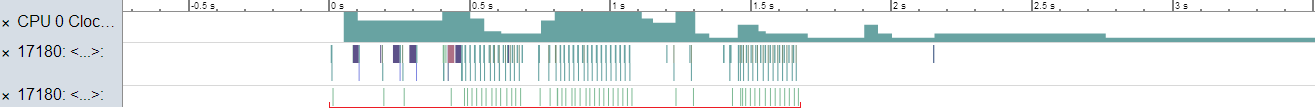
\includegraphics[width=0.9\textwidth]{resources/profiling/systrace/ub1events_non_optim.png}}
  \caption{Récupération et affichage des événements de l'université de Bordeaux 1 avant optimisation}
\end{figure}

L'élément qui nous a permis d'effectuer cette amélioration se trouve au niveau du \textit{layout} qui affiche la liste des événements récupérés. Après s'être renseigné au sein de la documentation Android, nous avons appris que la  modification de l'attribut booléen \textit{android:baselineAligned} à \textit{faux} au sein du \textit{layout} permet de gagner en performances en libérant l'application de la charge supplémentaire qu'elle avait à devoir aligner les \textit{baselines} des éléments fils.(Voir figure 8.2)

\begin{figure}[h!]
  \label{fig:systrace_optim}
  \center
  \setlength\fboxsep{5pt}
  \setlength\fboxrule{0.5pt}
  \fbox{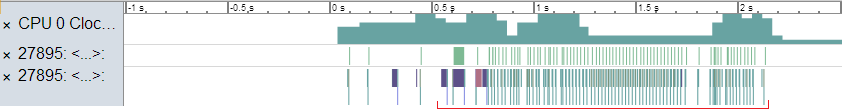
\includegraphics[width=0.9\textwidth]{resources/profiling/systrace/ub1events_optim.png}}
  \caption{Récupération et affichage des événements de l'université de Bordeaux 1 après optimisation}
\end{figure}

Comme on peut le voir sur l'enregistrement précédent, l'affichage des éléments se fait maintenant de manière nettement plus régulière que lors du premier enregistrement. L'optimisation de l'interface graphique a également permis une optimisation globale des performances de l'application puisque le temps d'exécution global(parsing et affichage) diminue automatiquement. 

\section{Method profiling}
Voici un tableau récapitulatif des temps d’exécution de nos fonctionnalités principales sur différents smartphones. Pour chacune d'elles, nous avons effectué des enregistrements qui montrent les temps d'exécution approximatifs des méthodes qui réalisent ces services. Les temps affichés correspondent donc au temps total d'exécution de nos threads appelés\textit{AsyncTask} qui représentent les tâches lourdes exécutes en arrière plan. Ces résultats sont approximatifs et peuvent varier étant donné que le temps d’exécution des méthodes dépend surtout de la fluidité de la connexion Internet utilisée.\\

\begin{table}[h]
\begin{adjustbox}{minipage=1.12\textwidth,margin=0pt \smallskipamount,center}
\begin{tabular}{|l|p{2.8cm}|p{2.8cm}|p{2.8cm}|}
	\hline
	~ & Samsung Galaxy S3 (1.4Ghz QuadCore CPU) & Sony Xperia S (1.5Ghz DualCore CPU) & LG Optimus 2X (1Ghz DualCore CPU) \\ \hline
	Evénements UB1 (RSS) & 1.4 sec & 1.5 sec & 1.7 sec \\ \hline
	Evénements LaBRI (RSS) & 2.1 sec & 2.3 sec & 2.4 sec \\ \hline
	Evénements LaBRI (HTML) & 1.7 sec & 1.7 sec & 1.7 sec \\ \hline
	Annuaire UB1 & 0.3 sec & 0.7 sec & 0.6 sec \\ \hline
	Annuaire LaBRI & 2.0 sec & 2.1 sec & 2.2 sec \\ \hline
\end{tabular}
\end{adjustbox}
\end{table}

Le temps obtenu pour le chargement des événements de l'Université de Bordeaux 1 est d'environ de 1.5 secondes(cf. figure 12.1), ce qui respecte largement les trois à quatre secondes indiquées dans le cahier des charges. Cela est du au fait que les événements de l'Université de Bordeaux 1 correspondent uniquement à des flux RSS à récupérer, ce qui représente une tâche peu couteuse et qui s'exécute relativement vite.
En ce qui concerne l'abonnement au LaBRI, les événements sont récupérés de deux manières distinctes en fonction de la catégorie demandée. Ils pourront donc être récupérés soit via les flux RSS soit en parsant directement les pages HTML du site web. Cela explique alors le temps plus long (2.1 secondes) nécessaire au chargement des actualités du LaBRI sachant que le parsing de pages HTML est plus couteux qu'une simple récupération de flux RSS étant donné qu'il y a une grande quantité d'événements à parcourir, dont certains datant d'il y a plusieurs années. Dans tous les cas, on respecte toujours largement le temps évoqué dans le cahier des charges avec un temps d'exécution tout à fait correct. (cf. figure 12.2)\\\\
 

La recherche dans l'annuaire de l'Université de Bordeaux 1 s'effectue de manière quasiment instantanée: 0.3 sec pour une première recherche (cf. figure 12.3). Cela est du au fait qu'on utilise une authentification auprès de l'annuaire de Bordeaux 1 en utilisant le protocole LDAP qui nous permet d'avoir une réponse rapide de la part du serveur. De plus, et étant donné que nous sommes limités par le serveur quand au nombre de résultats retournés suite à une requête (dix résultats maximum), l'utilisation du système \emph{Simple paged result control} nous permet de demander au serveur une page de résultats contenant donc dix contacts au maximum. Cela nous évite donc de surcharger le serveur et nous permet d'avoir sa réponse plus rapidement. L'utilisation d'un \emph{Connection pool} nous permet également de maintenir plusieurs connexions actives simultanément auprès du serveur LDAP, et donc de diminuer le temps de retour des requêtes lors de recherches successives dans l'annuaire. (moins de 0.2 secondes lors de la deuxième requête). Il est à noter que le temps de réponse peut varier en fonction de l'état du serveur LDAP de Bordeaux 1 qui peut être plus ou moins occupé à un moment précis.\\\\

Etant donné que les contacts du LaBRI sont récupérés à l'aide du parsing HTML, il est évident qu'ils prennent plus de temps à être parcourus que ceux provenant de l'Université de Bordeaux 1 (cf. figure 12.4) En effet lorsqu'on effectue une requête auprès d'un serveur LDAP, on recherche uniquement la tranche de l'annuaire correspondant à la recherche effectuée, alors que dans le cas du parsing de l'annuaire du LaBRI, on parcourt la totalité des contacts présents sur la page HTML et on renvoie uniquement ceux correspondants aux critères de recherche. Cela explique donc les temps supérieurs de la recherche de contacts lorsqu'on est abonné au LaBRI (environ 2 secondes) qui découlent de la complexité accrue de l'algorithme d'analyse textuelle effectué lors de chaque requête. Cependant, ces deux secondes représentent un temps plus que correct qui est toujours suffisamment petit pour ne pas avoir d'impact sur l'expérience utilisateur.


\section{Thread tracking}
Grâce à cet outil, nous avons pu observer en temps réel l’activité des threads exécutés par notre application. Après avoir analysé plus précisément leur comportement pour chacun des services proposés, nous avons pu remarquer un défaut dans notre implémentation de la recherche dans l’annuaire de l’université de Bordeaux 1. A chaque fois que nous effectuons une recherche auprès du serveur LDAP, nous nous connections de nouveau auprès du serveur sans réutiliser la connexion précédemment établie. Nous pouvions alors constater (voir code et figure ci-dessous) qu’à chaque fois qu’une nouvelle recherche était effectuée (représentée par le thread AsyncTask), un nouveau thread ConnectionReader  était crée pour se ré-authentifier inutilement au serveur LDAP.

\begin{figure}[h!]
  \label{fig:without_pool_code}
  \center
  \setlength\fboxsep{5pt}
  \setlength\fboxrule{0.5pt}
  \fbox{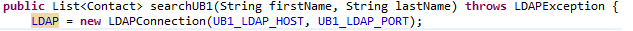
\includegraphics[width=0.9\textwidth]{resources/profiling/code_screenshots/code_without_pool.png}}
\end{figure}

\begin{figure}[h!]
  \label{fig:without_pool}
  \center
  \setlength\fboxsep{5pt}
  \setlength\fboxrule{0.5pt}
  \fbox{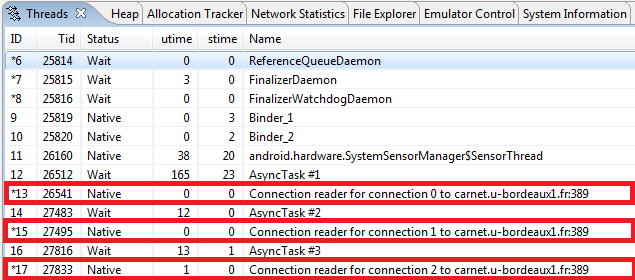
\includegraphics[width=0.9\textwidth]{resources/profiling/code_screenshots/threads_without_pool.png}}
\end{figure}

Cela nous a donc permis de rectifier ce problème en faisant en sorte de réutiliser l’authentification déjà existante, mais également d’apporter une optimisation en se servant de «pools de connexion» qui servent à maintenir plusieurs connexions établies auprès du serveur (10 au maximum),  et qui peuvent être réutilisées par plusieurs threads.\\
On se retrouve donc à présent dans une situation où lorsqu’on effectue plusieurs recherches consécutives dans l’annuaire de Bordeaux 1, un seul thread ConnectionReader est créé pour établir la connexion, et les AsyncTask correspondants aux recherches réutilisent la connexion établie au préalable (voir code et figure ci-dessous).

\begin{figure}[h!]
  \label{fig:with_pool_code}
  \center
  \setlength\fboxsep{5pt}
  \setlength\fboxrule{0.5pt}
  \fbox{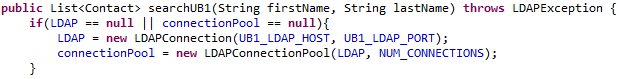
\includegraphics[width=0.9\textwidth]{resources/profiling/code_screenshots/code_with_pool.png}}
\end{figure}

\begin{figure}[h!]
  \label{fig:with_pool}
  \center
  \setlength\fboxsep{5pt}
  \setlength\fboxrule{0.5pt}
  \fbox{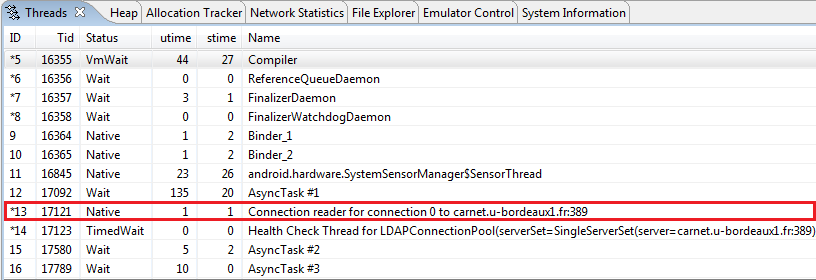
\includegraphics[width=0.9\textwidth]{resources/profiling/code_screenshots/threads_with_pool.png}}
\end{figure}

\newpage

\section{Network statistics}
L’outil d’analyse de paquets transitant sur le réseau à également été une statistique intéressante qui nous a permis de déterminer que notre application n’est pas en état de saturer un réseau, et de vérifier qu’elle n’est pas trop gourmande vis à vis du trafic de données.\\
D’après les analyses effectuées (Voir figure 8.3), lorsqu’on est connecté en Wi-Fi à un réseau haut débit (ADSL dans le cas de notre test), et qu’on récupère la totalité des événements (abonné à l'université de Bordeaux 1 et au LaBRI), le réseau est utilisé pendant environ 7 secondes et de manière discontinue ce qui l’empêche d’être saturé. Durant ces quelques secondes, l’application reçoit en moyenne 57 Ko de données pour afficher la totalité des informations nécessaires, ce qui est relativement une petite quantité de données qui ne pose aucun problème pour être récupérée même sur des connexions à plus faible débit tels que les réseaux mobiles (3G, EDGE, GPRS). 

\begin{figure}[h!]
  \label{fig:network_statistics_events}
  \center
  \setlength\fboxsep{5pt}
  \setlength\fboxrule{0.5pt}
  \fbox{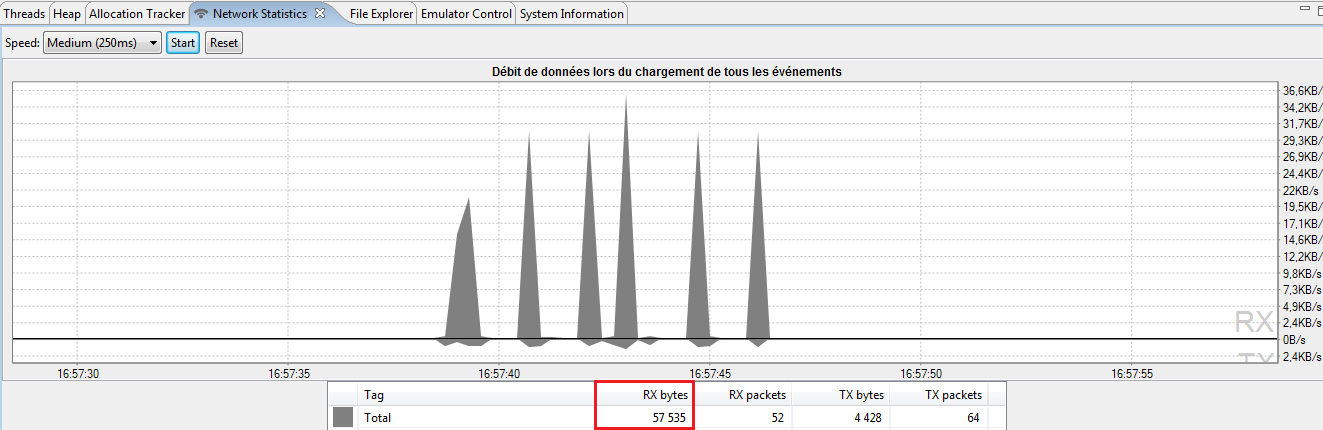
\includegraphics[width=0.9\textwidth]{resources/profiling/network_statistics/events.png}}
  \caption{Utilisation du réseau lors de la récupération de la totalité des événements du LaBRI et de Bordeaux 1}
\end{figure}

Il en est de même pour l’utilisation de l’annuaire (Voir figure 8.4) où la quantité de données à récupérer est encore plus faible (environ 26 Ko) et varie de façon minimale en fonction de la recherche effectuée. 

\begin{figure}[h!]
  \label{fig:network_statistics_directory}
  \center
  \setlength\fboxsep{5pt}
  \setlength\fboxrule{0.5pt}
  \fbox{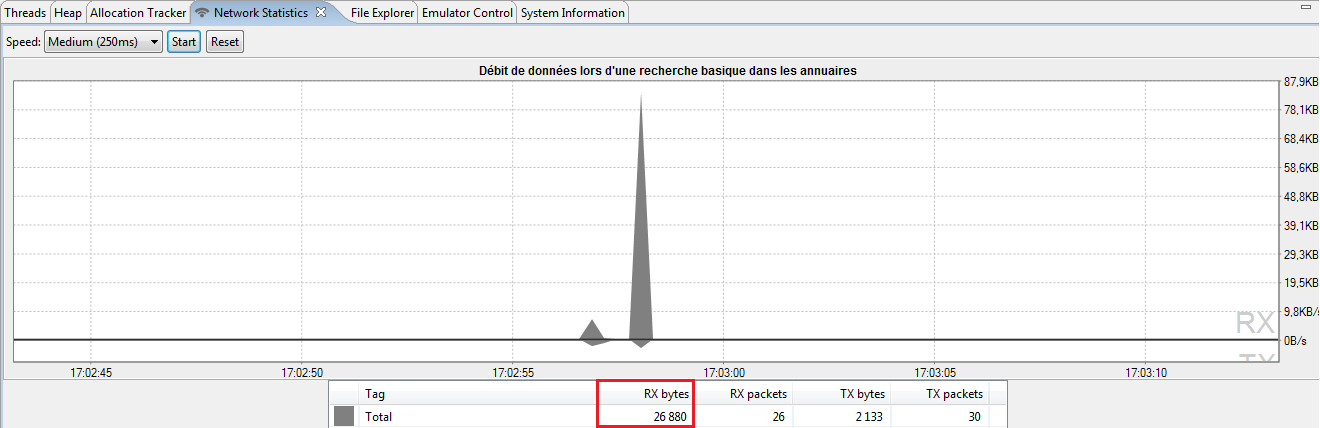
\includegraphics[width=0.9\textwidth]{resources/profiling/network_statistics/directory.png}}
  \caption{Utilisation du réseau lors d'une recherche basique dans les deux annuaires à la fois}
\end{figure}

Ces éléments prouvent que notre application est apte à tourner de manière optimale sur des supports mobiles divers, utilisés en extérieur lorsqu’une connexion haut débit ne se trouve pas forcément à proximité.